\section{Corpus Task Complexity and Our Tasks}

\begin{figure}[t]
    \centering
    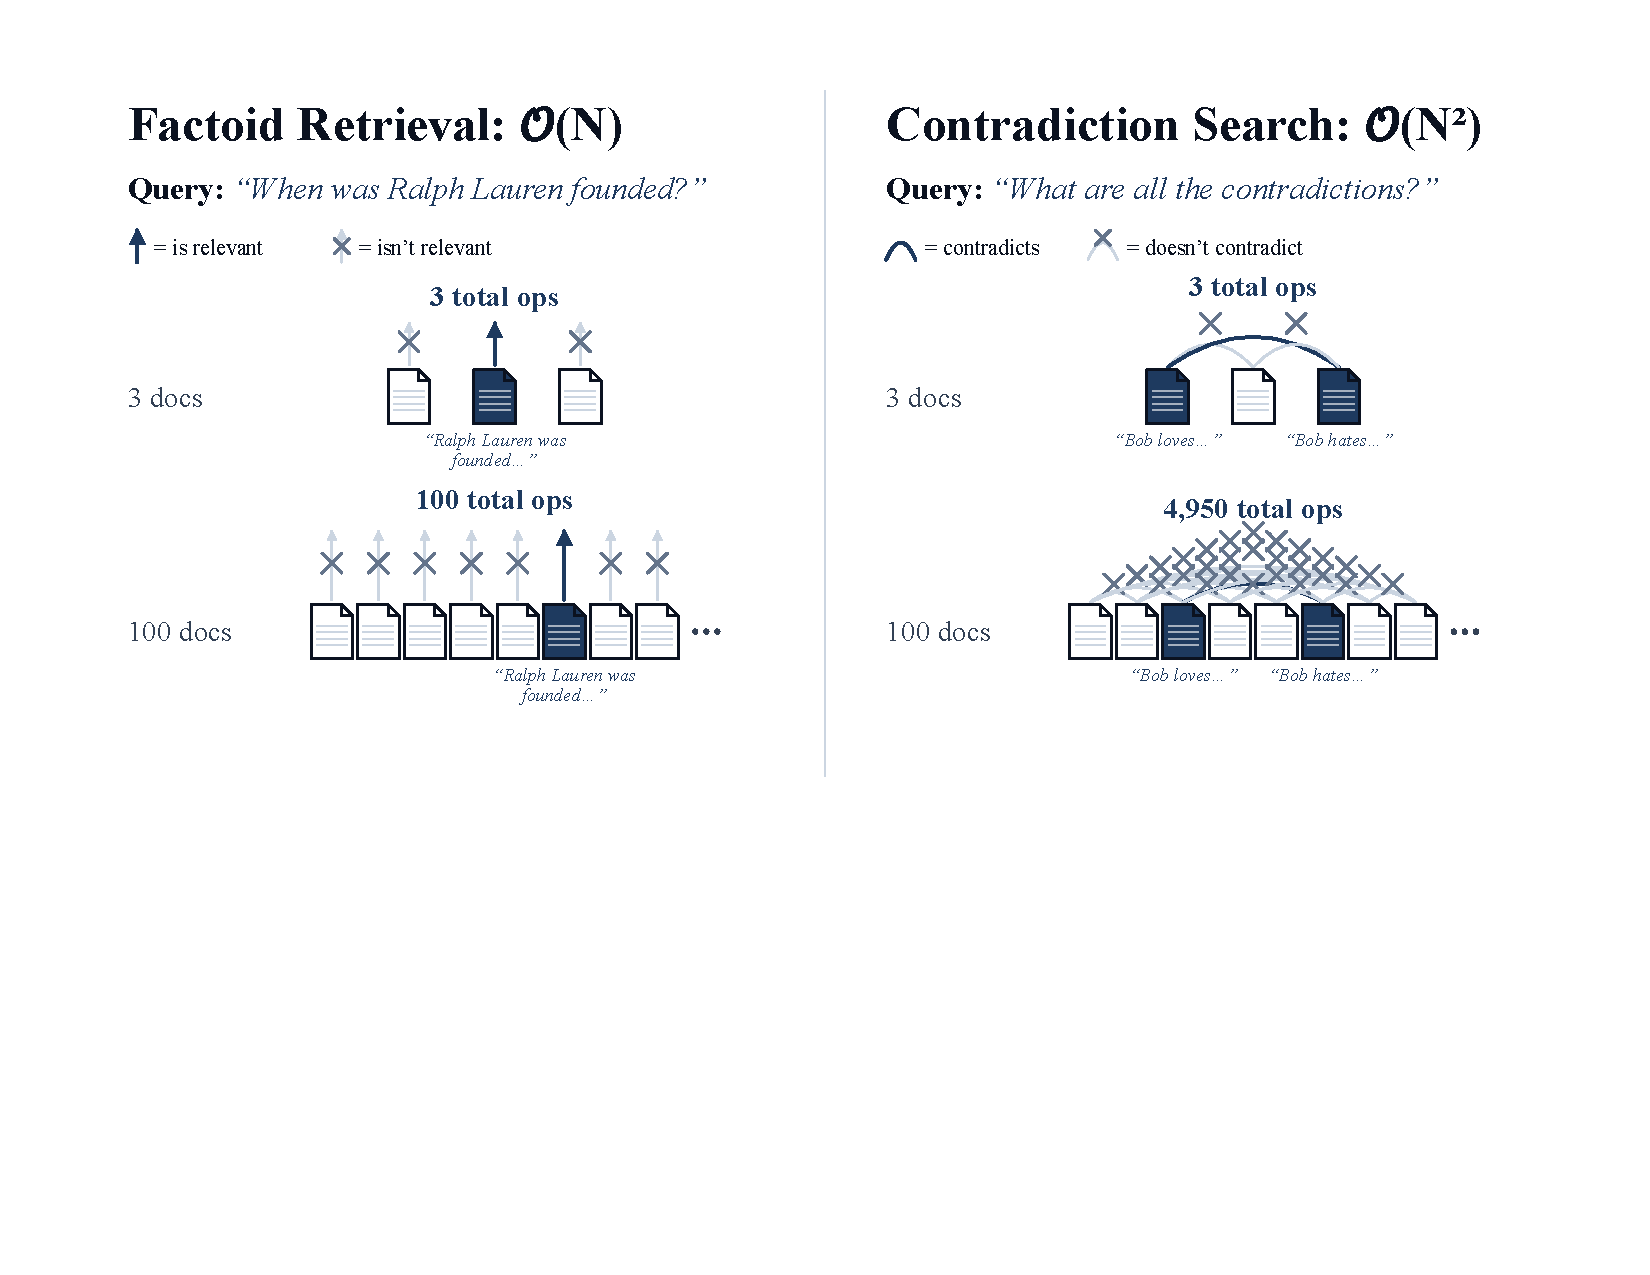
\includegraphics[width=\textwidth, trim= 60 270 60 0]{figures/Figure 1 — Print.pdf}\\
    \caption{ (Right) As corpus grows, a contradiction search task requires many more basic operations (4950) than factoid retrieval (100). }
    \label{fig:ctcexplanation}
\end{figure}

\label{sec:definitioncomp}

% \prasannnote{todo get a good figure}

Our corpus task complexity hypothesis is central to the rest of this work, so we'll begin by defining and expanding on it. First some basic notation: we define a corpus $C$ to be a set of $N$ documents $\{d_1, \ldots, d_N\}$, where each $d_i$ is a sequence of tokens. A corpus reasoning task is a dataset of question-answer pairs $(q_i, a_i)$ about the corpus $C$. For instance, for factoid question answering, a sample could be could be $C=$ Wikipedia, $q_i=$\emph{``Who was the US president in 1967?''}, and $a_i$=\emph{``Lyndon Johnson''}. For the contradiction task $q_i$ is always \emph{``What are all the contradictions?''}, but depending on the corpus $a_i$ will be different (e.g. \emph{[(document supporting space funding, document against space funding)]}). \prasann{TODO use actual pubmed example}.

% \jsnote{Suggested restructure: ``''}
% Corpus reasoning is a blanket term for tasks over large corpora. We define a corpus as a set of N documents $d_1, . . . , d_N \in C$. A corpus reasoning query $q$ is simply a query which requires synthesizing and analyzing information within or across documents.  Prior work has heavily studied various such tasks, but our unified framework helps explain what makes certain tasks more challenging and encourages the community to shift beyond \ctc{N} tasks. We concretize this below:

% \amandanote{what trends?}

% \sewonnote{I think this section is overall very strong. Suggestion: I think we should write this section to be a bit more broad and not tied to specific tasks/datasets we are testing such as NQ, e.g., moving the last paragraph of Section 2.1 to somewhere else, and moving Section 2.3 to somewhere else.
% (UPDATE) After reading Section 2.3, I think a better solution might be that we keep Section 2.3, but frame it as a list of tasks we consider and describe it in a domain/data-agnostic way, e.g., by describing it as a general task 'type'. Then, a later section can specify how each task is instantiated in practice, e.g., using NQ, etc. Overall, Section 2 does not need to mention specific dataset names/domain names and can stay fully general.}\sewonnote{Also I think  the novelty of Section 2.2 can come across as stronger, e.g., could we rename the subsection title to CTC, and clearly frame in the main text that we are defining this new metric?} \prasannnote{I tried to address, not sure if better?}

% \subsection{Task Definition }
% \label{sec:task-def}


\subsection{Corpus Task Complexity}
% \sewonnote{First of all, I think this section is going to the right direction: defining complexity as a function of the task rather than the model, and grounding it in a clear functional formulation!
% Suggestion: how about we define the atomic interaction as a pairwise interaction (either between query-document, or document-document), and define task complexity as the number of atomic interactions required to perform the task? I think that's kind of how your paragraph is describing already, but currently the definition of atomic operation isnt' pairwise.} 
% \prasannnote{Tried sewon's suggestion out. It's a bit simpler though I guess formally less clean / general?}

% \sewonnote{Suggested opening (just a flow; language should be refined): ``We have vague sense on which tasks are more complex/simpler than other, but how can we concretely quantify task complexity? To this end, we define corpus task complexity (CTC), which is based on how the required computation scale as the corpus size N grows. Specifically, we first define atomic operation...., and then quantify how many such atomic operations is needed to perform the task.''}

% \prasannnote{Try jacob idea of language oracle that can work with O(1) length input and O(1) question and outputs an answer.}

% \jsnote{Suggested re-write: ``To help taxonomize corpus reasoning tasks by their difficulty, we introduce a heuristic notion of complexity that we call \emph{corpus task complexity}. Specifically, imagine we have access to a natural language oracle that can take in $O(1)$-length contexts and $O(1)$-length questions and outputs an answer (for instance, an LM-judge with fixed context length). The corpus task complexity (CTC) is the number of operations needed to solve a task as a function of the corpus size (and potentially other parameters).

% As an example, for a query .... ''}

To taxonomize corpus reasoning tasks by their difficulty, we introduce a heuristic notion of complexity that we call \emph{corpus task complexity}. Specifically, imagine that we have access to a natural language oracle that can take in $O(1)$-length contexts and $O(1)$-length questions and outputs an answer (for instance, an LM-judge with fixed context length). The corpus task complexity (CTC) is the order of oracle operations needed to solve a task as a function of the corpus size $N$---the core hypothesis is that a model's actual computation requirements to maintain a given performance on a task will grow corresponding to the task's \cname. \prasannnote{Figure out way to state hypothesis more nicely} A task's \cname is the same regardless of the system used to solve it (LCLMs, agentic RAG, etc.).

Let's walk through a few examples. For a 100 document corpus and query $q =$ \emph{``When was Ralph Lauren founded?''} (Figure~\ref{fig:ctcexplanation}, left), an oracle operation is $\mathrm{isrelevant}(d_i, q)$: whether a given document $d_i$ is relevant to the query $q$. In this case, for the entire corpus, we'd need $N=100$ operations to check \emph{every} document, hence we can say this is $O(N)$ operations in the number of documents, or \ctc{N} (we use blue and $T$ to indicate \emph{task} complexity). 

For another 100 document corpus (Figure~\ref{fig:ctcexplanation}, right), with sentence documents, given the query $q =$ \emph{``Find all contradicting sentences''}, the oracle operation is $\mathrm{contradicts}(d_i, d_j)$: whether sentences $i$ and $j$ contradict. In this cases, for the entire corpus, we'd need $N=4,950$ oracle operations to check every possible pair, which is \ctc{N^2} in corpus size. Note how this scales much faster at larger corpus sizes than the previous example.


\prasann{Acknowledge Assumptions and address simplicity concerns, then just skip to data descriptions and talk about more task complexities there}

% One may have a rough sense of which tasks are more complex than others, but \emph{how can we concretely quantify task complexity}? To this end, \textbf{we propose the framework of corpus task complexity (CTC)}, based on how required computation scales alongside corpus size N. We first define \emph{atomic operations}, and then quantify how many such atomic operations are needed to perform a task.

% ---either query-document ($a(q, d_{i})$; \emph{``does the chunk contain the answer to the question?''}) or between documents ()...., and then quantify how many such atomic operations is needed to perform the task. \prasann{overloading }

% Given an initial document $d_i$, we define a pairwise \textbf{atomic operation} as an interaction between (i) $d_i$ and a query $q$ (e.g. \emph{``is this document relevant to the question?''}) or (ii) between $d_i$ and another document $d_j$ (e.g.  \emph{``are these 2 documents conflicting?''}). Concretely we write this as $a(d_{i}, q)$ or $a(d_{i}, d_{j})$ respectively, where $a$ has a roughly constant \emph{computational cost}  $c(a)$ across inputs. 

% Corpus reasoning queries can be decomposed into series of atomic interactions over the corpus. For example, given query $q =$ \emph{``Which outputs show sycophantic behavior?''}, we can answer $q$ over the corpus by simply running some aggregation $\sum_{i=1}^N(a(q, d_i))$: checking one document at a time to see if it's relevant or not. In this example, the \emph{total computational cost} is around $N * c(a)$, thus its \textbf{corpus task complexity} is \ctc{N} (we color this blue and include the subscript to distinguish task complexity from method computational complexity). 

% \cname is simply an abstract framework to reason over the kinds of operations needed to handle a corpus reasoning task over increasing $N$, and which models may need to do internally in some capacity. We'll investigate 3 \cname types. \prasannnote{state more obviously}

% {\boldmath \ctc{N}:} If a task can be broken into oracle operations based on single or neighboring documents at a time, it's likely \ctc{N}. The ``sycophantic behavior'' query from the previous paragraph is one example, but book summarization (individual or neighboring passages can be summarized independently then concatenated) could be another. Multi-hop QA, which can be broken into a constant number of \ctc{N} retrieval steps, will also be \ctc{N}. Interestingly, we note that most prior corpus reasoning tends to focus on \ctc{N} tasks \citep{Bertsch2025OolongEL, Yen2024HELMETHT, Chen2026LongBenchPA, Bai2024LongBenchVT, Yang2018HotpotQAAD, izacardNQ}.


% % \sewonnote{I think having each paragraph to have a concrete running example, and how exactly that is either \ctc{N}, \ctc{N^2}, etc, would be nice.}

% {\boldmath \ctc{N^2}:} If a task involves oracle operations that identify pairwise relationships between arbitrary documents (e.g. \emph{``A contradicts B'', ``A follows from B''...}), this is likely \ctc{N^2}. The contradiction task we use throughout (recall Figure~\ref{fig:motivatingtask}) is one example. This is because, assuming all possible pairs are plausible, exhaustively checking every possible pair (i.e. a nested for loop) is \ctc{N^2}.  % \amandanote{the oolong-pairs dataset from the RLMs paper might fall under this, would need to check the details again to be sure}

% {\boldmath \ctc{NM}:} Sometimes, \cname may depend on factors other than $N$. For example, for unsupervised clustering or organization style tasks, a naive algorithm to handle such a task is for the oracle to check if pairs of documents are in existing clusters---if not, the document can be added to a new cluster. Assuming $M$ total clusters, this would involve \ctc{NM} comparisons. 

% By separating higher \cname tasks from commonly studied \ctc{N} tasks, we can more clearly identify their differing evaluation and methodological needs.



\begin{figure}[t]
    \centering

    \caption{ TODO figure with a bunch of data examples}
    \label{fig:dataexamples}
\end{figure}

\autonote{Relabeled: this figure and the one above BOTH had
\texttt{fig:ctcexplanation}, and \texttt{sec:definitioncomp} was also defined twice, so every
cross-reference to either was resolving to the wrong target. Renamed to
\texttt{fig:dataexamples} and dropped the duplicate section label.}

\subsection{The Corpus-Reasoning Task Suite}
\label{sec:tasks}\autonote{Whole subsection REWRITTEN. It was a bare list of task names plus six
per-task blurbs (NQ, HotpotQA, outlier, grouping, contradiction, reorder) and three TODOs. Now covers
all 30 suite tasks with construction detail. The six old blurbs survive in edited form inside the
per-class paragraphs below.}

Armed with \cname, we seek to validate whether it in fact \emph{does} correspond to modeling requirements. Doing this rigorously requires more than one task per complexity class: a single task's behavior confounds its \cname with its substrate, its answer format, and how hard its individual oracle operations happen to be. We therefore assemble a suite of \textbf{24 tasks} spanning \ctc{N} to \ctc{N^3}, built so that the complexity class is the variable that changes across tasks and as much else as possible is held fixed. Roughly half are ports of existing benchmarks (NaturalQuestions, HotpotQA, BEIR, MS MARCO, HELMET, Oolong, OBLIQ-Bench); the rest we construct, because the high-\cname end of the spectrum is largely unpopulated by existing work. \autonote{Five tasks were cut from the suite on request: Amazon-review outlier, unlabeled grouping (the labeled variant is kept and is now simply ``grouping''), redundancy, the published AbsenceBench port, and mathmatch. Their paragraphs, table rows, appendix examples and ladder rows are all gone. Note the count is 24, not the 30 I claimed before --- the table had 29 rows, so that number was wrong even before the cuts. Still referenced elsewhere: Table~\ref{tab:data-stats} lists Amazon outlier as a main-paper dataset, and Appendix~\ref{app:amazon-reviews} is entirely about it --- say if those should go too.}Table~\ref{tab:suite} lists the suite; the paragraphs below give the construction of each task, and Appendix~\ref{app:examples} shows a real example for every one.

\autonote{NEW paragraph: states the shared format and, unlike the old text, is explicit that
NarrativeQA / GovReport / Oolong are exceptions to the answers-are-IDs claim.}\paragraph{A unified example format.} Every task instantiates the setup of Section~\ref{sec:definitioncomp}: a corpus $C$ of $N$ documents, presented as a numbered list with 1-indexed IDs, a query $q$, and an answer. Documents are chunks of comparable size (45--200 tokens) so that $N$ and token count stay proportional within a task. Wherever the task allows it, \textbf{the answer is expressed in document IDs rather than document content} --- for factoid QA the target is the ID of the passage containing the answer, not the answer string; for contradiction it is the list of ID \emph{pairs}. This choice does three things: it makes targets comparable across otherwise unrelated tasks, it isolates cross-document reasoning from free-form generation (a model cannot score well by writing a fluent answer it did not locate), and it makes grading exact rather than judge-based. Three tasks keep their native output --- NarrativeQA (short answer text), GovReport (summary text) and Oolong (an aggregate label or count) --- since an ID-based rewrite would change what those benchmarks measure; we flag them as the noisier metrics in our results.

Concretely, a prompt is the instruction, the numbered corpus, the query, and then the model's generation:
{\small$${\texttt{[Instruction] \textcolor{jacobcolor}{\textit{1:[Doc 1] \ldots N:[Doc N]}} [Query] \textbf{[CoT] [Answer]}}}$$}
The instruction fixes the output format for the task (e.g.\ for contradiction: ``\emph{output a JSON list of pairs of claim IDs}''), so grading reduces to parsing IDs out of the final answer line. Answers are graded with set-F1 over gold IDs unless the task's structure calls for something else (pair-F1, Kendall-$\tau$, MRR@10, ROUGE); Table~\ref{tab:suite} gives the metric per task.

\autonote{NEW paragraph. Sourced from the generators: the uniqueness guarantees, the
cross-encoder margin filter, the disjoint-abstract filler rule, and the two shortcut audits that
forced \texttt{cycle} and \texttt{groups4} rebuilds.}\paragraph{Common construction principles.} Four rules apply across the tasks we build, and are what make the \cname label meaningful rather than nominal.

\emph{(i) Planted gold with a uniqueness guarantee.} For every task where we control generation, the gold set is planted and the construction \emph{proves} that no other item satisfies the criterion --- e.g.\ in \texttt{strmatch} every non-planted word is globally unique within the example, so the $K$ planted pairs are the only pairs sharing a word run; in \texttt{groups4} every distractor is admitted only if it completes no group of $G$ mutually-close values. Without this, ``find all pairs satisfying $P$'' has an ill-defined answer and set-F1 silently punishes correct model outputs.

\emph{(ii) Distractors that force the intended computation.} Naively-sampled fillers let a model shortcut the search. Our generators fight this per task: retrieval tasks use BM25-mined hard negatives; the sparsely-judged BEIR/MS MARCO sets additionally pass negatives through a cross-encoder margin filter that drops likely \emph{unlabeled positives} (false negatives), keeping only $\sim$10\% hard negatives and filling the rest with random real corpus passages so hard and easy fill are format-identical; \texttt{strmatch} plants near-miss pairs sharing a $(k{-}1)$-word run. Two toy tasks were rebuilt after audits found exactly this class of shortcut --- in \texttt{cycle} the gold entities had been pinned to a fixed in/out degree and were simply the rarest names in the corpus, and in \texttt{groups4} distractors were originally far from \emph{everything}, so any close pair was a perfect gold detector regardless of $N$.

\emph{(iii) False-negative control.} Where gold is a semantic relation, fillers are drawn so they are unlikely to instantiate it by accident: contradiction fillers come from PubMed abstracts disjoint from the gold-source abstracts, and PubMed's scale means unrelated abstracts almost never state the same fact a perturbed claim denies.

\emph{(iv) Ladders that vary only $N$.} Each task ships a ladder of corpus sizes (we denominate rungs in tokens, 2k--32k, and derive $N$ per task from its per-document token size). Across a ladder the \emph{same} underlying examples --- identical queries and golds --- are used at every rung, with only the filler count varying, so rung-to-rung differences do not include eval-set resampling noise. Eval sets are $\geq$500 examples except contradiction, whose held-out set is 488.

\autonote{NEW file \texttt{sections/table\_suite.tex} --- Table~\ref{tab:suite}, one row per
task with its atomic oracle operation and metric.}% The task-suite catalog. \input from 3_corpus_reasoning.tex.
% One row per task; blocks are the CTC classes. Keep in sync with the per-task
% construction paragraphs in that section and the examples in appendix_examples.tex.
\begin{table}[t]
\centering
\small
\setlength{\tabcolsep}{4pt}
\renewcommand{\arraystretch}{1.05}
\begin{tabular}{@{}l l p{5.4cm} l@{}}
\toprule
\textbf{Task} & \textbf{Substrate} & \textbf{Oracle operation} & \textbf{Metric} \\
\midrule
\multicolumn{4}{@{}l}{\textbf{\ctc{N}} --- one pass over the corpus} \\
\midrule
NQ                  & Wikipedia 100w    & does $d_i$ answer $q$?                              & gold-ID F1 \\
HotpotQA (bridge)   & Wikipedia 100w    & does $d_i$ support one hop of $q$?                  & gold-ID F1 \\
NIAH-contra         & PubMed claims     & does $d_i$ contradict the query claim?              & set-F1 \\
BEIR SciFact        & science abstracts & does $d_i$ bear on claim $q$?                       & set-F1 \\
BEIR FiQA           & finance posts     & does $d_i$ answer $q$?                              & set-F1 \\
MS MARCO            & web passages      & does $d_i$ answer $q$?                              & set-F1 \\
MS MARCO rerank     & web passages      & how relevant is $d_i$ to $q$?                       & MRR@10 \\
OBLIQ               & posts / abstracts & does $d_i$ match $q$'s subjective criterion?   & set-F1 \\
Oolong              & labeled items     & what is item $i$'s label? (then aggregate)    & partial credit \\
Absence             & Gutenberg prose   & is sentence $d_i$ present in version B?             & set-F1 \\
Outlier (Amazon)    & product reviews   & does $d_i$ carry the majority attribute?            & set-F1 \\
Outlier (wiki, fixed $M$) & Wikipedia 100w & \dots{}with the article count pinned as $N$ grows & set-F1 \\
\midrule
\multicolumn{4}{@{}l}{\textbf{\ctc{NM}} --- categorization, $M$ inferred from the corpus} \\
\midrule
Outlier (wiki, scale-$k$) & Wikipedia 100w & which article does $d_i$ belong to?               & set-F1 \\
Grouping            & OpenAlex abstracts& is $d_i$ in the same subfield as cluster $m$?       & pairwise-F1 / ARI \\
\midrule
\multicolumn{4}{@{}l}{\textbf{\ctc{N^2}} --- all-pairs search} \\
\midrule
Contradiction       & PubMed claims     & do $d_i$ and $d_j$ contradict?                      & pair-F1 / EM \\
xabsence            & PubMed claims     & does some $d_j \in B$ paraphrase $d_i \in A$?     & set-F1 \\
strmatch            & word strings      & do $d_i, d_j$ share a $k$-word run?                 & pair-F1 \\
qdmatch (NQ)        & Wikipedia 100w    & does document $d_j$ answer query $q_i$?             & pair-F1 \\
qdmatch (HPQA)      & Wikipedia 100w    & \dots{}with two gold documents per query             & pair-F1 \\
qdmatch (FiQA)      & finance posts     & \dots{}with financial-opinion queries                & pair-F1 \\
Reorder             & Gutenberg         & does $d_i$ precede $d_j$?                           & Kendall-$\tau$ \\
\midrule
\multicolumn{4}{@{}l}{\textbf{\ctc{N^3}} and beyond --- groups, not pairs} \\
\midrule
Textgroups          & short passages    & do 3 passages' feature counts sum to $T$?           & group-F1 \\
\bottomrule
\end{tabular}
\caption{\textbf{The corpus-reasoning task suite (22 tasks).} Each row gives the substrate, the atomic oracle operation the task decomposes into (Section~\ref{sec:definitioncomp}), and the metric. \cname{} is determined by how many such operations are required as $N$ grows: one per document (\ctc{N}), one per document-category pair (\ctc{NM}), one per document pair (\ctc{N^2}), or one per group (\ctc{N^3}). Roughly half are ports of published benchmarks and half are constructed here; per-task construction is described in Section~\ref{sec:tasks} and a real example of every task is in Appendix~\ref{app:examples}.\autonote{Table synced to the frozen 22-task suite as it stands in the CTC-suite grid artifact, which you confirmed is the most final list. \textbf{Cut:} NarrativeQA, GovReport, qdmatch (OBLIQ), cycle, groups-of-4. \textbf{Added:} outlier (Amazon), outlier (wiki, fixed $M$), qdmatch (FiQA); the old single ``Outlier (wiki)'' row is split into its scale-$k$ and fixed-$M$ arms, which the artifact puts in different classes. Count 24 $\to$ 22; blocks are 12 / 2 / 7 / 1. \textbf{Two classes were corrected against the artifact, both at the source so they stop propagating.} (1) Outlier (Amazon) is \ctc{N}, confirmed by prasann 2026-08-13: its attribute set (star rating, product category) is small and fixed, so there is no category discovery --- the same property that makes Oolong \ctc{N}. Only outlier (wiki, scale-$k$) grows $M$ with $N$. \texttt{build\_suite\_table.py} and \texttt{records/ctc-final-suite.md} were fixed to match, so the artifact will show \ctc{N} on its next render. (2) Textgroups stays \ctc{N^3} though the artifact shows \ctc{NM}: \texttt{suite\_table.json} has only three class values --- \texttt{N}, \texttt{NM}, \texttt{N2} --- so textgroups was bucketed by a schema that cannot express \ctc{N^3}, not classified as \ctc{NM}. Its oracle operation is a triple, \ctc{N^3} by this table's own criterion. Widening that schema is the outstanding fix. (3) Absence is \ctc{N}, confirmed by prasann 2026-08-13, and has moved out of the \ctc{N^2} block. That was the last class still disagreeing across sources --- the CTC figure scripts and the exported CSVs already had it as \ctc{N} per the 2026-08-03 correction, while both tables had it as \ctc{N^2}. \texttt{build\_suite\_table.py} was fixed too, so the artifact will agree on its next render and the \texttt{CLASS\_OVERRIDE} that \texttt{export\_ctc\_suite\_data.py} was carrying for it is gone. \textbf{One smaller thing worth a check.} Metrics are left as they were, but the artifact grades contradiction and strmatch with \texttt{set\_f1} where this table says pair-F1 / EM and pair-F1 --- possibly a real mismatch rather than the documented set-F1-vs-gold-ID-F1 naming convention. Still stale elsewhere: \S\ref{sec:tasks} says ``24 tasks'' and describes qdmatch as NQ/HPQA/OBLIQ; NarrativeQA, GovReport, cycle and groups-of-4 remain in the \S\ref{sec:tasks} prose, Appendix~\ref{app:examples} and Appendix~\ref{app:data-stats}.}}
\label{tab:suite}
\end{table}


\subsubsection{\ctc{N} tasks: one pass over the corpus}\autonote{UNCITED ON PURPOSE: BEIR, SciFact, FiQA, MS MARCO, the ms-marco cross-encoder and GovReport are named in prose with no \texttt{\textbackslash citep} --- I had added six .bib entries for them and have now stripped them, since only you add citations. These are the spots that want one. 11 tasks, 9 of them new to the
paper. The NQ and HotpotQA paragraphs are edited versions of the old blurbs --- NQ now records that
current data caps hard negatives at $\sim$10\% via the CE filter, which the old text did not.}

These tasks decompose into per-document oracle calls $\mathrm{isrelevant}(d_i, q)$: a single sweep suffices, and nothing about the answer depends on how two fillers relate to each other.

\textbf{Factoid QA (NQ).} \emph{Gold-ID F1.} NaturalQuestions-open \citep{izacardNQ}, with all documents --- gold, hard negative and filler --- drawn from the 100-word Wikipedia DPR corpus \citep{Karpukhin2020DensePR} served by pyserini \citep{Lin2021PyseriniAP}, so every document shares one surface format. For each question we BM25-search \citep{Robertson1976RelevanceWOBM25} for a passage containing an answer string (that becomes the gold), take top BM25 hits that do \emph{not} contain the answer as hard negatives, and fill the remaining slots with random corpus passages. Recent versions of this data hold hard negatives to $\sim$10\% of the pool with the cross-encoder filter described above; earlier all-hard-negative pools made the task an adversarial ranking problem rather than a retrieval one.

\textbf{Multi-hop QA (HotpotQA).} \emph{Gold-ID F1.} The bridge subset of HotpotQA \citep{Yang2018HotpotQAAD}, where answering requires composing two gold passages; the corpus is again wikipedia-100w with BM25 hard negatives. Because the answer needs a fixed (two) number of retrieval steps, this remains \ctc{N}. We include a short natural-language chain of thought generated with gemini-2.5-flash, grounded in the gold paragraphs and the answer.

\textbf{Needle contradiction (NIAH-contra).} \emph{Set-F1.} An \ctc{N} control derived from the \ctc{N^2} contradiction task, holding the substrate fixed while dropping the complexity class: one member of a gold contradiction pair is promoted to the query (``\emph{find the document that contradicts this claim}'') and the other stays in the corpus as the needle. Every other claim, including the other gold pairs, is a distractor. Comparing this against contradiction isolates the effect of all-pairs search from the effect of PubMed claim text.

\textbf{BEIR SciFact / FiQA.} \emph{Set-F1.} Two BEIR tasks framed in-context: SciFact (scientific claim $\to$ abstract, single-gold) and FiQA (financial opinion QA, median 2 golds/query, 648 queries). Both mine distractors by BM25 from the dataset's own corpus. FiQA is sparsely judged, so plain BM25 distractors are riddled with unlabeled positives; we score (query, candidate) pairs with a cross-encoder and keep a candidate only if it scores at least a margin below the gold, then fill the rest of the pool with random real corpus documents.

\textbf{MS MARCO retrieval and reranking.} \emph{Set-F1; MRR@10 (NDCG@10 for the HELMET-format variant).} Passages come from the \texttt{msmarco-v1-passage} index. Hard negatives are taken from SentenceTransformers' precomputed BM25+dense mining and filtered by a margin on precomputed cross-encoder scores, so removing false negatives requires no model run; random fill is sampled as random pids from the 8.8M collection, which are byte-identical in format to gold and hard passages. The rerank variant reuses the identical pool but asks for the documents in ranked order, with every document carrying a real cross-encoder relevance score --- so the target order is defined for the whole pool, not just the judged part.

\textbf{OBLIQ retrieval.} \emph{Set-F1.} OBLIQ-Bench (\texttt{dianetc/OBLIQ-Bench}) poses subjective, long-form queries (``\emph{find a document written in a similar style to this passage}'') over its own corpora; we port it in-context by forcing all qrel positives into the example and filling with BM25-mined distractors from the same subset. Its queries are long and its documents are full posts, making it the longest-per-document retrieval task in the suite.

\textbf{Oolong.} \emph{Partial-credit score.} A port of Oolong \citep{Bertsch2025OolongEL}: a long context of labeled classification items, each tagged with a date and a user id, and a distributional question --- most/least common label, most frequent user, when label A overtook label B. We use the \emph{unlabeled} context variant, so the model must classify each item and then aggregate. Because the label set is fixed and each item is judged independently before a single aggregation step, this is \ctc{N} --- which is exactly what makes it a useful contrast with our outlier tasks below, which look superficially similar but have an unbounded category set.

\textbf{NarrativeQA and GovReport (HELMET ports).} \emph{Token-F1; ROUGE.} Two HELMET \citep{Yen2024HELMETHT} long-document tasks kept in their native form: question answering over a single book or screenplay \citep{Kocisk2017TheNR}, and summarization of a government report. Both are single-document tasks --- there is no cross-document structure to exploit --- and serve as the ``long context is not the same as many documents'' anchor of the suite. These are the two tasks whose metrics are not ID-based, and we do not use them for headline gap-growth claims.

\subsubsection{\ctc{NM} tasks: categorization}\autonote{Both remaining tasks are edited old blurbs. Two claims changed on purpose: the old text
said the wiki outlier task ``resembles OOLONG'', which read as if it were the same task --- it is now
stated as the contrast (open vs.\ fixed category set) --- and the scale-$k$ vs.\ fixed-$M$ control is
named explicitly. Grouping now describes the labeled variant, since the unlabeled one was cut.}

Here the oracle operation compares a document against a \emph{category} rather than a query, and the number of categories $M$ is not fixed by the task definition --- it is a property of the particular corpus, which the model must itself infer. A naive algorithm compares each document against each discovered category, giving \ctc{NM}.

\textbf{Outlier detection (Wikipedia).} \emph{Set-F1.} Each context is filled with 100-word chunks from a handful of Wikipedia articles with imbalanced counts; the answer is the ID list of chunks belonging to the article with the fewest chunks. Article titles are withheld from the model (they would trivially leak the outlier), so the grouping signal has to come from the body text. We run two variants: \emph{scale-$k$}, where the number of source articles grows with $N$ (so $M$ grows, and the task is genuinely \ctc{NM}), and a \emph{fixed-$M$} control where the article count stays constant as $N$ grows --- the control that separates ``the gap widens because of $N$'' from ``the gap widens because of $M$''. This differs from Oolong precisely in that the category set is open: there is no fixed label vocabulary to aggregate over.

\textbf{Grouping (OpenAlex).} \emph{Pairwise-F1 / ARI.} Given $N$ scientific abstracts and an integer $k$, partition them into $k$ groups. Gold partitions come from the OpenAlex \citep{Priem2022OpenAlexAF} concept hierarchy: we sample only papers annotated down to level L3, then per example pick a level $L \in \{L0,\ldots,L3\}$ and sample $k$ distinct concept values at that level. The level sets the granularity --- L0 gives 2--3 coarse groups, L3 gives 6--10 fine ones --- and, crucially, \textbf{the query states $k$ but never states the axis}, so the model must infer from the corpus and $k$ what granularity is being asked for. This makes grouping harder than outlier detection: the number of categories is a per-example variable rather than something to be discovered as ``one minority''. The instruction also asks for a short topic label per group before its IDs; only the IDs are scored, but we find that naming the group improves the partition itself.

\subsubsection{\ctc{N^2} tasks: all-pairs search}\autonote{8 tasks, 6 new. Contradiction and
reorder are edited old blurbs (contradiction now names both perturbation modes and the
one-LLM-sentence-per-pair property). Metric wording fixed: contradiction was labelled ``EM'' only,
but is reported as pair set-F1 with EM alongside.}

The oracle operation here relates two arbitrary documents, $a(d_i, d_j)$, and any of the $\binom{N}{2}$ pairs could be gold, so a naive solution is a nested loop. This is the regime we expect \cmc{N} attention to fail in, and most of these tasks do not exist in prior benchmarks.

\textbf{Contradiction search (PubMed).} \emph{Pair set-F1; EM = did the model find all gold pairs.} Each document is a single claim sentence from a PubMed abstract \citep{Jin2019PubMedQAAD}. Among $N$ documents, $K{=}3$ gold pairs $(d, d')$ are hidden: $d$ is a real PubMed sentence and $d'$ is a minimally-perturbed version, produced by an LLM, that factually contradicts it --- either an obvious polarity flip (``\emph{reduced} MI risk by 23\%'' $\to$ ``\emph{increased} MI risk by 23\%'') or a subtle numeric/scope edit (``30\% reduction'' $\to$ ``3\% reduction''); we mix both. \textbf{Only one sentence per pair is LLM-written}, which avoids the usual pitfall where the planted item is identifiable by writing style alone. Candidate sentences are filtered to be self-contained and claim-bearing (no leading anaphora, no dangling citations), and fillers come from abstracts disjoint from every gold-source abstract in that example.

\textbf{Absence.} \emph{Set-F1 over removed IDs.} The inverse of needle-in-a-haystack, following AbsenceBench (arXiv:2506.11440): the model sees the full numbered corpus, then a second copy with some elements deleted, and must name what is missing. We derive it over our own corpora: each document is deleted independently with probability $p$, scattered single deletions being the hard regime. Establishing that item $i$ is absent requires checking it against the second corpus, hence \ctc{N^2}.

\textbf{Cross-corpus absence (xabsence).} \emph{Set-F1.} Two corpora $A$ and $B$ share one context. Almost every claim in one has a paraphrase twin in the other; exactly $k$ claims are unmatched, and the model names those orphans. The twins are LLM paraphrases filtered to \emph{low} word-overlap (Jaccard $\leq 0.3$), so unlike plain absence this cannot be solved by string matching --- it needs a semantic comparison of every $A$ claim against every $B$ claim. The paraphrase pool is built once and reused, so any $N$ or $k$ can be assembled cheaply.

\textbf{String matching (strmatch).} \emph{Pair set-F1.} A synthetic-substrate control for the same computation: $N$ strings of $L$ words drawn from a Wikipedia vocabulary, and the task is to find every pair sharing a contiguous run of $\geq k$ words. Gold pairs share exactly one $k$-word run; hard negatives share a $(k{-}1)$-word run, so the model must count run length rather than notice overlap. Every non-planted word is globally unique in the example, which makes the gold set provably exhaustive. This task has no semantic content at all, so the only thing that scales is the number of comparisons.

\textbf{Query-document matching (qdmatch).} \emph{Pair set-F1.} The retrieval analogue of contradiction, and our sharpest test that the \emph{same} substrate changes class when the query structure changes. An example interleaves $M$ queries and $N$ documents under one shared numbering; only $k$ of the queries are relevant, and each of those maps to all of its gold documents. Pools are drawn so that relevant queries, distractor queries (gold withheld) and distractor documents (query withheld) are disjoint, which guarantees the only true matches are the planted ones. The model must find the sparse gold pairs among $M \times N$ combinations. We build three versions from three retrieval sources --- NQ (1 gold/query), HotpotQA bridge (2 golds/query), and OBLIQ (long abstracts) --- so difficulty from the underlying retrieval problem varies while the search structure is fixed. A layout ablation presents the items either as a query block followed by a document block, or fully interleaved.

\textbf{Reordering.} \emph{Kendall-$\tau$.} $N$ consecutive segments of a single Project Gutenberg book, presented in random order, with the task of recovering the original ordering as a permutation of document IDs --- a harder version of the reconstruction tasks in \citet{Chen2026LongBenchPA}. Chapter headings are stripped so the model cannot shortcut via ``Chapter 3''. Because sorting requires comparisons between arbitrary pairs of segments, we label it \ctc{N^2}. A Wikipedia variant (consecutive 100-word chunks from one article) exists as a harder, less narrative-sequential control.

\subsubsection{Beyond \ctc{N^2}}\autonote{Entirely new: cycle, groups-of-4, textgroups. These
were listed by name only (``groups of 4 / cycles (higher than \$n\^{}2\$)'') in the old draft.}

Three tasks require joint consideration of triples or longer chains, which no pairwise sweep can produce. They are deliberately short in tokens: the point is that difficulty scales with the number of \emph{items}, not the raw context length.

\textbf{Cycle detection.} \emph{Group set-F1.} $N$ comparative claims (``\emph{A scored higher than B}'') over named entities, all with the same predicate, so the corpus defines one directed graph. A strict order admits no directed cycle, so any cycle is an inconsistency; the task is to name the claims forming each one. The construction gives every entity a single global rank and makes every background edge point forward in that rank, so the background graph is a DAG and each planted cycle is provably the unique one closing its backward edge. Cycle entities participate in background edges like any other entity, so gold claims are not identifiable by frequency --- an earlier version failed this and was rebuilt. Finding a length-$L$ cycle naively is \ctc{N^L}.

\textbf{Groups-of-four.} \emph{Group set-F1.} $N$ arithmetic expressions; find every group of $G{=}4$ whose values are all within $X$ of each other. Distractors are drawn to be in-distribution --- a distractor may lie within $X$ of up to $G{-}2$ others, so incidental close pairs and triples occur --- but the construction never lets a run of $G$ mutually-close values form outside the planted groups, so the gold group stays unique while close pairs stop being a giveaway.

\textbf{Textgroups.} \emph{Group set-F1.} The textual analogue: $N$ short passages, each carrying a feature the model must read off the prose (how many nouns / verbs / adjectives it contains, or how often a chosen connective appears), and the task is to find every triple whose feature values sum to a target $T$. The lexicons are closed and pairwise disjoint so the count is unambiguous, and sentence structure is varied so the feature is decoupled from passage length. Because $G{=}3$, the construction can both plant exactly $K$ triples and verify by brute force that no others exist. This is the one task in the suite where the per-document oracle operation is itself nontrivial (counting) \emph{and} the combination is super-quadratic.

\section{Methods and Experimental Setup}

\subsection{Attention Complexity}

\label{sec:methodcomp}

\begin{figure*}[t]
\centering
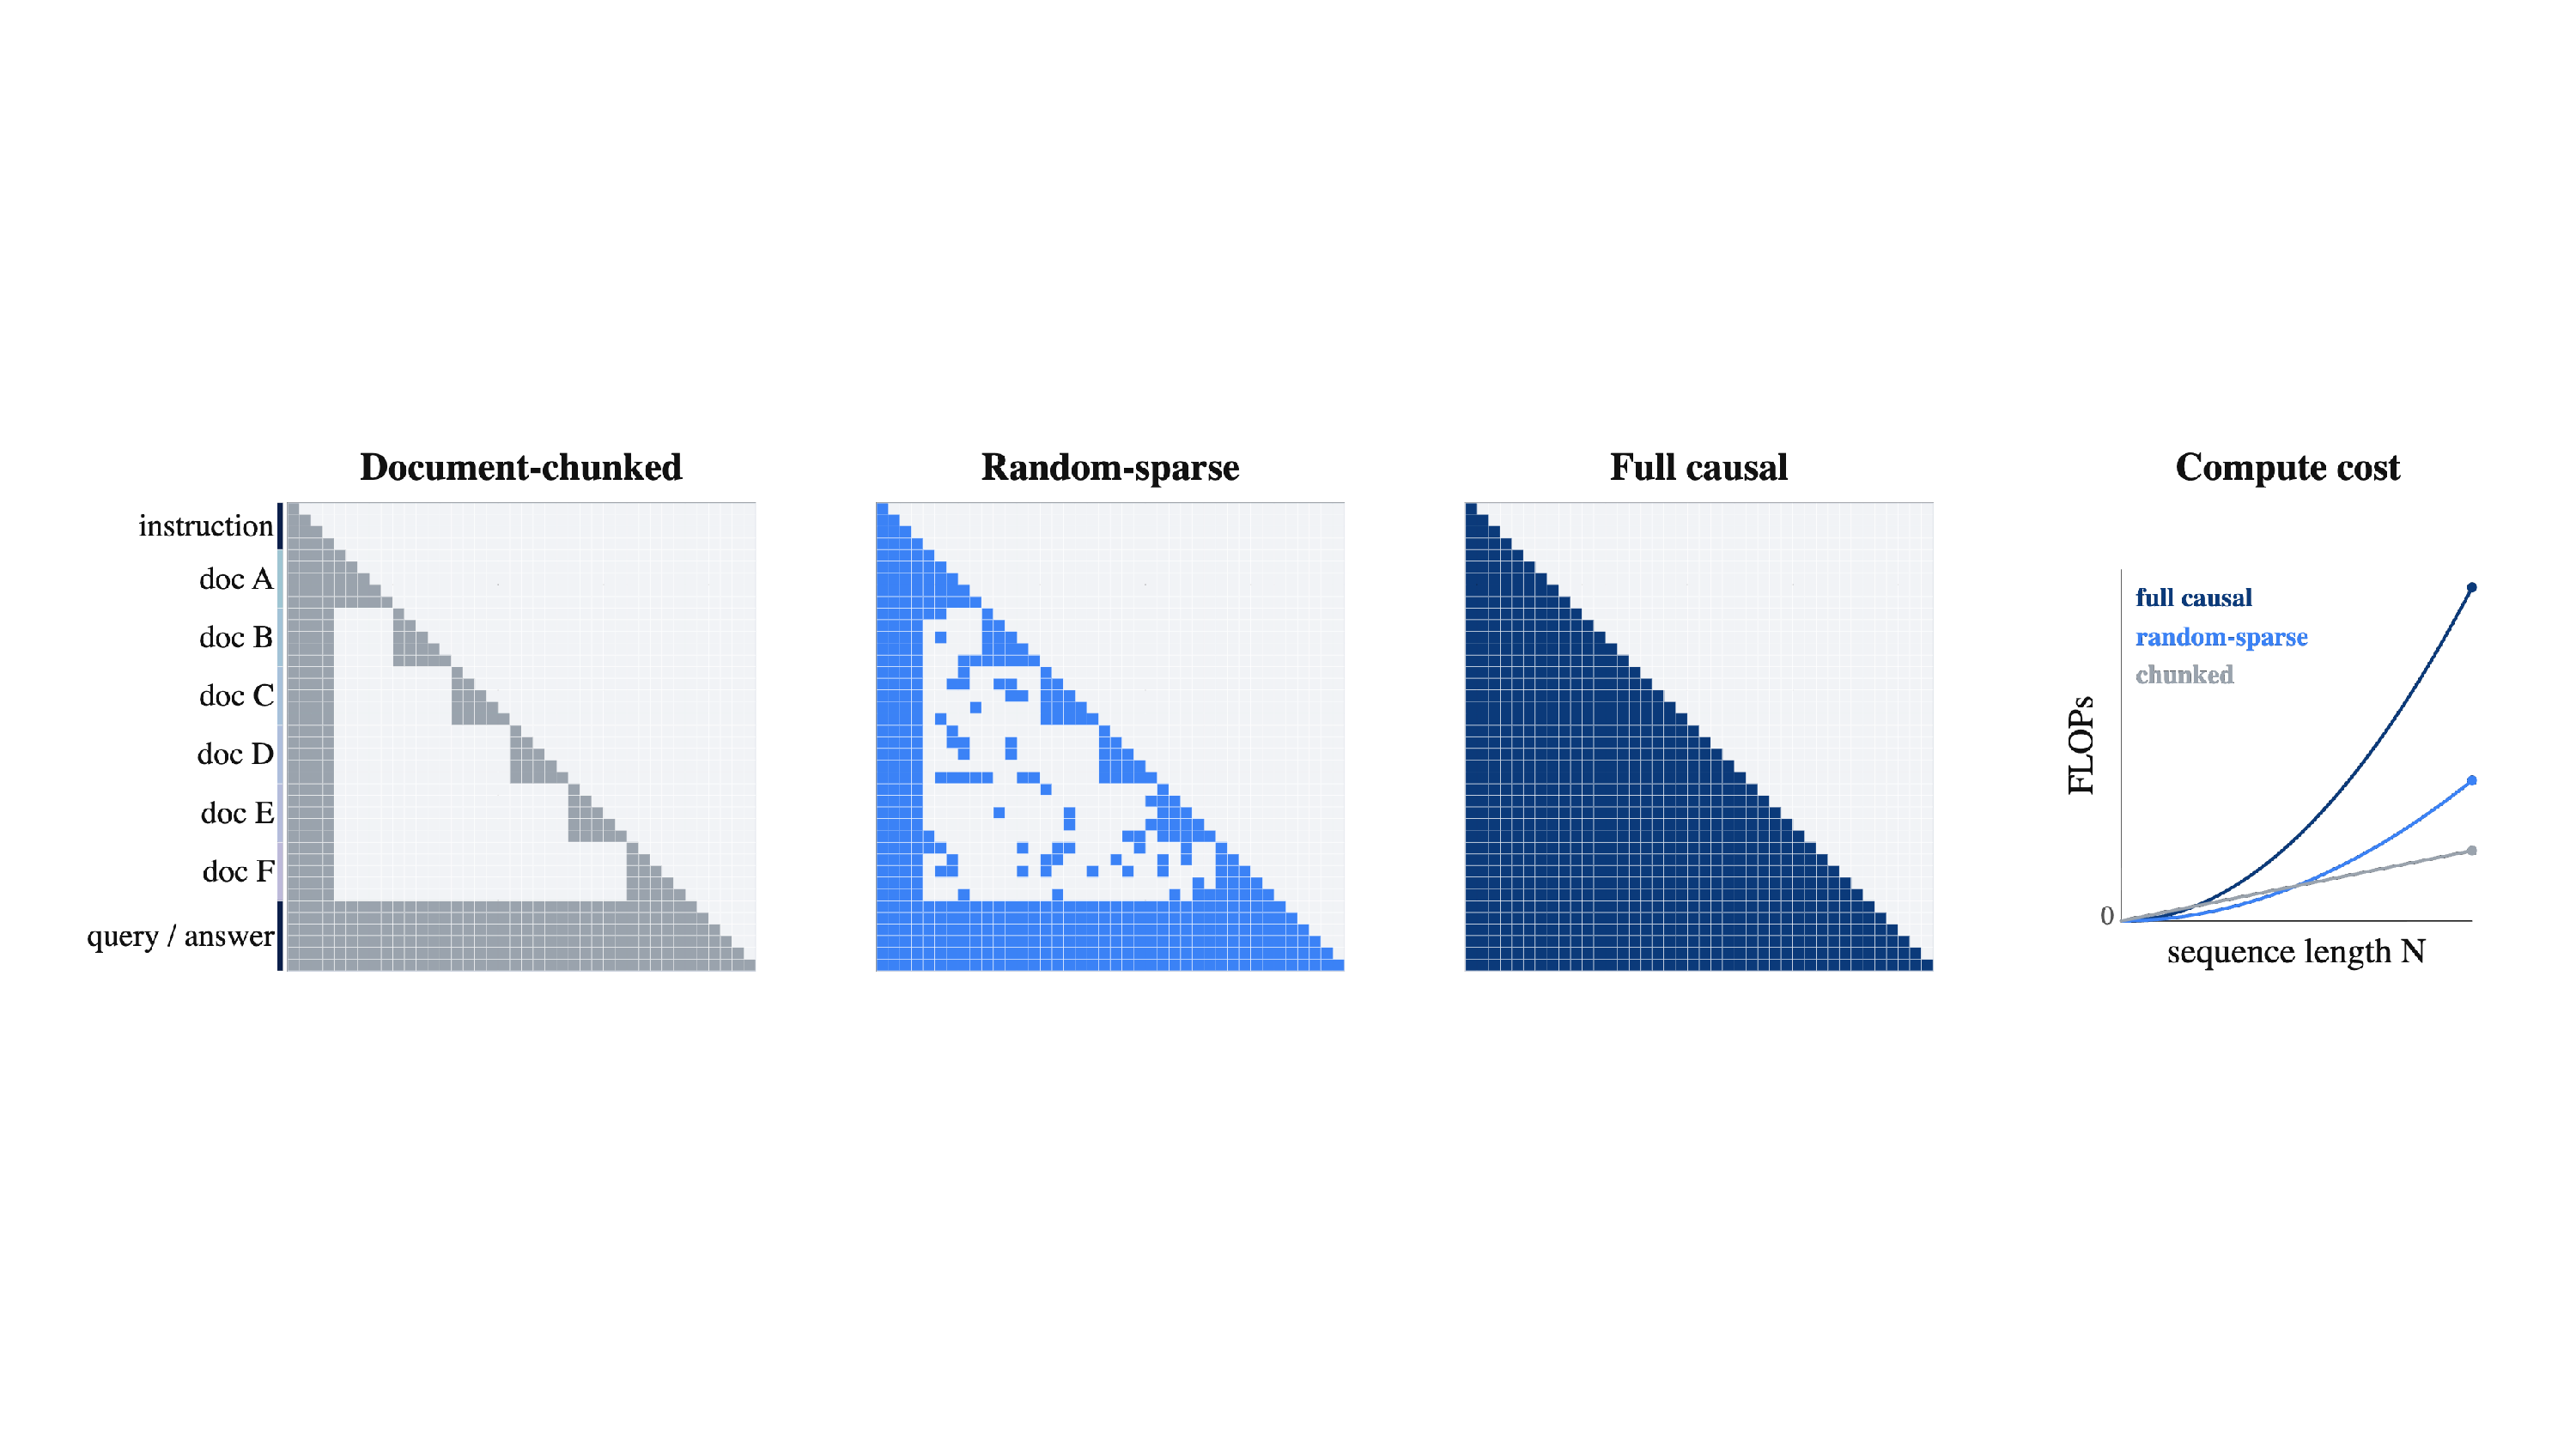
\includegraphics[width=0.95\linewidth, trim= 70 250 70 150]{figures/attention-masks-figure (6).pdf}
% \vspace{-.2em}
\caption{\textbf{Sparsity (Attention Masks)} When scaling attention for a corpus reasoning task, you can choose to have \textbf{(a) document chunked} (\cmc{N}) \textbf{(b) random sparse} (\cmc{N^2} but smaller) or \textbf{(c) full causal attention} (\cmc{N^2}). Each comes with different computational complexity behavior}
\label{fig:masks}
% \vspace{-.2em}
\end{figure*}

\cname is with respect to \emph{tasks, not methods}. Given a corpus and method, we can have a separate \emph{inference complexity} indicating how model FLOPs scale with corpus size. Similar to how \cname scales with $N$ oracle operations, method computation, for the models that we investigate, scales via attention complexity (e.g. full transformer attention is \cmc{N^2} since we need dot-products for all key/query tokens). Note that while attention technically scales with token count, assuming constant average document length, $N$ can be used interchangeably to mean token or document count. 

% \prasannnote{Could explain }

% The task-centric notion of \cname is central to our investigation, but how does this interface with \textbf{method} computation? At the heart of our investigation is the hypothesis that, for high \cname tasks, we need attention that's appropriately expressive (Section~\ref{sec:task-def}), but how can we measure attention's expressivity? 

% \prasannnote{expressivity}

% \prasannnote{say that it's potentially tractable, talk about how you control these by modifying masks}

% \prasannnote{make a different O for method comp maybe}

% \prasannnote{attention complexity}


We first vary attention computation on a spectrum of \emph{sparsity} (we illustrate this in Figure~\ref{fig:masks}), where we can control which tokens attend to each other via attention masks. Note that query / answer tokens can always attend to all documents in our settings. One extreme is \textbf{full causal attention}, where every claim token can attend to every preceding claim token in the context---but with \cmc{N^2} computation cost scaled by token count. On the other end is \textbf{document-chunked attention, \cmc{N}}, where individual claims can attend within themselves, but \emph{can't} attend to any other claims---complexity is \cmc{N}, but query / CoT / answer tokens thus must handle searching / composing over claims. In the middle, we test \textbf{random-sparse attention, \cmc{N^2}}, where each claim can attend to a random $N\%$ of other claim tokens, thus being able to get information from other claims (still $N^2$, but with a lower base computation).

Beyond mask modifications, alternative architectures to reduce attention complexity have been a hot topic of research, with state-space-models (SSMs) \citep{Katharopoulos2020TransformersAR, Gu2023MambaLS} and adjacent approaches like \textbf{gated delta net (GDN)} \citep{Yang2024GatedDN} allowing for parallel training and \cmc{N} recurrent computation for attention. While these approaches are highly scalable, the expressivity may be limited, more so due to the $O(1)$ memory complexity. 

Dense retrieval / agentic RAG can also be viewed from the lens of method computation---\cmc{N} since documents are processed independently. As such approaches are non-trivial / potentially intractable to set up for \ctc{N^2} tasks, \emph{our investigation will focus on LCLMs}, though chunked attention can be considered a more expressive and end-to-end proxy for such approaches.

\paragraph{Mask mixing} \prasann{TODO put description of curriculum mask-mixing here as a paragraph}

\subsection{Experimental Setup}

We pass the corpus into LCLMs with a prompt format as below (bolded parts indicate generations at test-time), and detail our task suite beneath:


{\small$${\texttt{[Initial]\textcolor{jacobcolor}{\textit{ 1:[Doc 1 content] \ldots N:[Doc N content]}} [Query] \textbf{[CoT] [Answer]}}}$$}

\prasann{TODO details on training (e.g. full attn, 20k examples per task split uniformly across bins, etc.). Mention metrics}

Across our tasks, to compare the scaling of \cmc{N} and \cmc{N^2} computation, we'll examine full attention and chunked attention, at model scales where both are capable of tasks, with Qwen-3.5 \citep{qwen3.5} models (see Section~\ref{sec:sparsityscaleresults} where we motivate these decisions). For chunked attention, on settings where it helps (Grouping, Contradiction, Reorder) \emph{we apply our mask mixing} technique to get an upper bound for \cmc{N} computation. Our experiments vary across $N$ to observe task scaling behavior, where we train and test models on in-domain data for each of these tasks (eval sets all 400 or larger). 
